\documentclass[a4paper, 12pt]{scrartcl}
\usepackage{listings}
\usepackage{color}
\usepackage{graphicx}
\usepackage{hyperref}
\lstdefinelanguage{XML}
{
  basicstyle=\ttfamily\footnotesize,
  morestring=[b]",
  moredelim=[s][\bfseries\color{blue}]{<}{\ },
  moredelim=[s][\bfseries\color{blue}]{</}{>},
  moredelim=[l][\bfseries\color{blue}]{/>},
  moredelim=[l][\bfseries\color{blue}]{>},
  morecomment=[s]{<?}{?>},
  morecomment=[s]{<!--}{-->},
  commentstyle=\color{black},
  stringstyle=\color{blue},
  identifierstyle=\color{red}
}

\setkomafont{sectioning}{\rmfamily}

\title{XML Technologies: Exercise 8}
\date{}
\subtitle{XML Design, RDF}

 
\begin{document}
\maketitle\vspace{-12ex}

\noindent This is a mandatory exercise and the result will be part of your final mark. The solution must be uploaded to OLAT by \textbf{May 20\textsuperscript{th} at 15:59}. Late submissions will not be accepted.\\


\noindent Submit the following files in a zipped archive:
\begin{itemize}
\item design.txt
\item rdf.xml
\end{itemize}

\noindent Make sure the archive is named [lastname]\_[firstname]\_8.zip (for example \textit{mueller\_mathias\_8.zip}). Some parts of your submission may be automatically evaluated, so make sure to name your files \textit{precisely} as prescribed, otherwise you might not get any points.

\section{XML Design}

After seeing many XML technologies put to good use (among others: DTD, XML Schema, XPath, XSLT) and since the semester is coming to an end, it is now time to take a step back. When looking at the very basics of XML, we intentionally skipped one crucial stage -- that is, how XML documents are designed in the first place.\\


\noindent XML design is a crucial step because any XML technology \textit{builds on top of it}. In other words, bad design has hardly anything to do with an intrinsic badness, it should be understood as hindering the processing of documents (navigation, query, transformation). In most cases, it's not that the design is bad \textit{per se}, but, considering the purpose is should serve, it is disadvantageous. \\

\noindent As a consequence, it is absurd to think about the design of an XML document if you have no idea what it (i.e. the document) is going to be used for. So, defining the purpose of XML actually precedes its design.

\subsection{Intelligent Design (2 points)} 

Imagine the following. You are working for a software company and currently in charge of overseeing the design of a new kind of XML document. It should serve the following purpose: \\

\noindent \textit{Represent information on countries. Specifically, the data should include the country and continent codes, the current population, the area it covers and last year's GDP. Several applications will access this document to retrieve information on specific countries. Therefore, e.g. retrieving the population of one specific country should be a trivial operation. On the other hand, given a GDP value, it should be simple to determine the respective country. } \\



\noindent Two members of the team you are leading have volunteered to devise a design (sample data taken from \url{http://countrycode.org/}). Both drafts are now subject to your thorough scrutiny. \\

\noindent \textbf{Draft A}

\lstinputlisting[language=XML]{attachments/draft_a.xml}

\vspace{0.5cm}

\noindent \textbf{Draft B} 

\lstinputlisting[language=XML]{attachments/draft_b.xml}

\noindent Both drafts can also be found in the exercise zip folder, as \texttt{draft\_a.xml} and \texttt{draft\_b.xml}. \\

\noindent \textbf{Study drafts A and B very closely. Decide which of the drafts is better suited for the task, given the requirements stated above. Do not rely on your intuition. \\ \\ Instead, substantiate your claim with XPath expressions that contrast the effort necessary to retrieve
\begin{itemize}
\item the population of one specific country
\item a country, using its GDP value as an identifier
\end{itemize}
given either draft A or B as the query document. Be as clear as possible, your bosses never underwent proper XML training.} \\

\noindent \textbf{Save your findings as \texttt{design.txt}. Include your choice of draft, an explanation in complete sentences and suitable XPath expressions.}

\section{RDF (3 points)}

The RDF standard is one of the most serious attempts to semantically enrich the web to date. It is meant to represent any kind of knowledge: facts, concepts and relationships. RDF is not limited to XML syntax, XML just happens to be one of the \textit{serialisation formats} of RDF. Another form of serialising an RDF network of knowledge is Notation3 (N3). \\

\noindent Yet another way of displaying RDF is a graph, where serialisation is not an issue, since all information can be shown simultaneously.\\

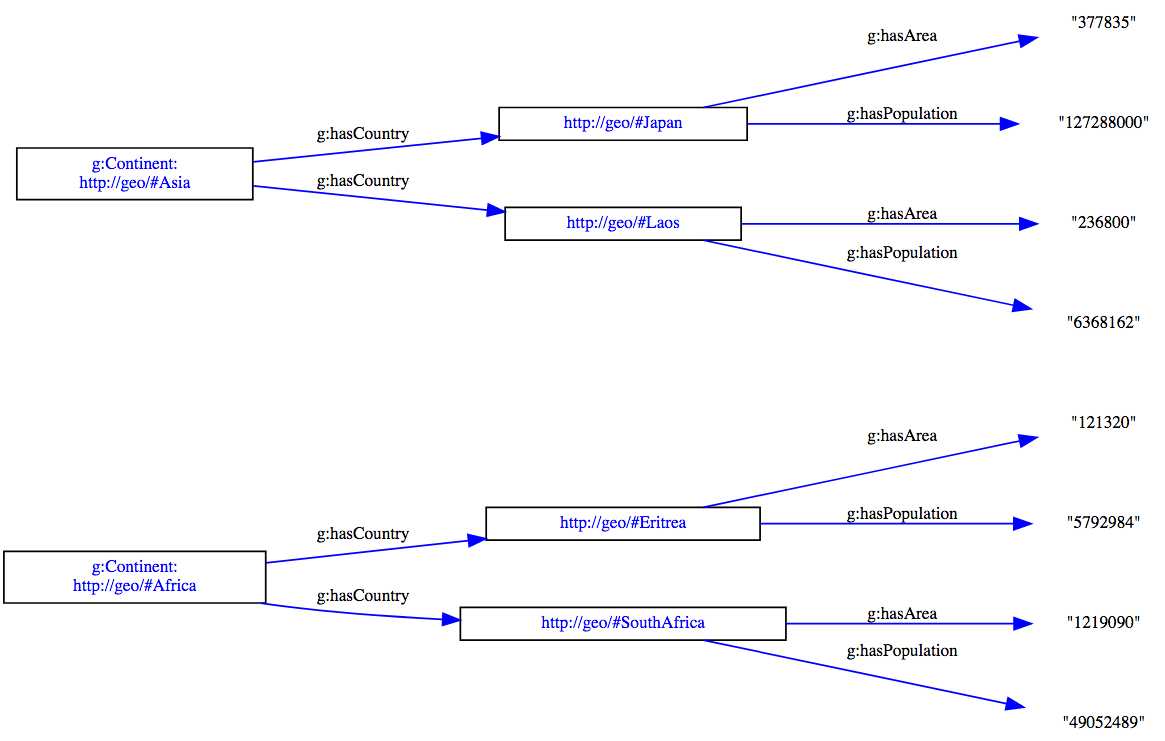
\includegraphics[width=17cm]{attachments/render.png}
\vspace{0.5cm}

\noindent Nodes in the graph represent objects and types, while arrows (predicates) indicate a relationship between nodes. As you can see, the kind of information displayed is similar to question 1 above. The graph is also available attached as \texttt{render.png}. \\

\noindent \textbf{Write a serialised version of the graph above that represents all information in XML RDF syntax. Declare two namespaces, one for RDF elements:}
\lstset{language=XML}
\begin{lstlisting}
xmlns:rdf="http://www.w3.org/1999/02/22-rdf-syntax-ns#"
\end{lstlisting}
\textbf{Another one for the domain-specific facts:}
\lstset{language=XML}
\begin{lstlisting}
xmlns:g="http://geo/#"
\end{lstlisting}
\textbf{The beginning and end of your document should look like:}
\begin{lstlisting}
<?xml version="1.0" encoding="UTF-8"?>
<rdf:RDF
    xmlns:rdf="http://www.w3.org/1999/02/22-rdf-syntax-ns#"
    xmlns:g="http://geo/#">
    <!--Your code here-->
</rdf:RDF>
\end{lstlisting}
\textbf{Use the official RDF XML validator\footnote{Online at \url{http://www.w3.org/RDF/Validator/}.} to validate your solution before submitting it. Also, the validation service is useful to learn how RDF translates to either model triples or graphs. Save your RDF as \texttt{rdf.xml}.}
\end{document}